%% REPLACE SXXXXXX with your student number
\def\studentNumber{S2570340}


%% START of YOUR ANSWERS
%% Add answers to the questions below, by replacing the text inside the brackets {} for \youranswer{ "Text to be replaced with your answer." }. 
%
% Do not delete the commands for adding figures and tables. Instead fill in the missing values with your experiment results, and replace the images with your own respective figures.
%
% You can generally delete the placeholder text, such as for example the text "Question Figure 2 - Replace the images ..." 
%
% There are 18 TEXT QUESTIONS (a few of the short first ones have their answers added to both the Introduction and the Abstract). Replace the text inside the brackets of the command \youranswer with your answer to the question.
%
% There are also 3 "questions" to replace some placeholder FIGURES with your own, and 3 "questions" asking you to fill in the missing entries in the TABLES provided. 
%
% NOTE! that questions are ordered by the order of appearance of their answers in the text, and not by the order you should tackle them. Specifically, you cannot answer Questions 2, 3, and 4 before concluding all of the relevant experiments and analysis. Similarly, you should fill in the TABLES and FIGURES before discussing the results presented there. 
%
% NOTE! If for some reason you do not manage to produce results for some FIGURES and TABLES, then you can get partial marks by discussing your expectations of the results in the relevant TEXT QUESTIONS (for example Question 8 makes use of Table 1 and Figure 2).
%
% Please refer to the coursework specification for more details.


%% - - - - - - - - - - - - TEXT QUESTIONS - - - - - - - - - - - - 



%% Question 1:
\newcommand{\questionOne} {
\youranswer{The figures 1a and 1b contain training + validation errors and training + validation accuracy for a baseline model on the EMNIST dataset, respectively. As the weights and biases get updated (as the iteration goes), the model's errors get lower and accuracy get higher (for both training and validation sets). This is the case for these specific figures for the first few iterations, before the validation error and accuracy deviate from the training, with the error getting even higher than the first iteration after ~40 iterations, and the accuracy gradually lowering, until after 100 iterations, they reach ~1.6 and ~0.81 for the validation error and accuracy, respectively. In constrast, the training error reaches a value close to 0 and the accuracy reaches >0.95. This is the case of overfitting, where the model fails to generalise for a wide variety of inputs.}
}

%% Question 2:
\newcommand{\questionTwo} {
\youranswer{Question 2 - Present your network width experiment results by using the relevant figure and table}
}

%% Question 3:
\newcommand{\questionThree} {
\youranswer{Question 3 - Discuss whether varying width affects the results in a consistent way, and whether the results are expected and match well with the prior knowledge (by which we mean your expectations as are formed from the relevant Theory and literature)}
}

%% Question 4:
\newcommand{\questionFour} {
\youranswer{Question 4 - Present your network depth experiment results by using the relevant figure and table}
}

%% Question 5:
\newcommand{\questionFive} {
\youranswer{Question 5 - Discuss whether varying depth affects the results in a consistent way, and whether the results are expected and match well with the prior knowledge (by which we mean your expectations as are formed from the relevant Theory and literature)}
}





%% Question 6:
\newcommand{\questionSix} {
\youranswer{Question 6 - Explain the experimental details (e.g. hyperparameters), discuss the results in terms of their generalisation performance and overfitting. Select and test the best performing model as part of this analysis.}
}

%% Question 7:
\newcommand{\questionSeven} {
\youranswer{Question 7 - Assume you were able to run 8 further training instances (8 specific hyperparameter configurations) where you could combine Dropout and L1, and/or Dropout and L2 regularisation. Which 8 runs would you pick and what question(s) would you aim to answer? Make sure you define the experiment setup, including any relevant hyperparameters}
}



%% Question 8:
\newcommand{\questionEight} {
\youranswer{Question 8 - Briefly draw your conclusions based on the results from the previous sections (what are the take-away messages?), discussing them in the context of the overall literature, and conclude your report with a recommendation for future directions}
}

%% - - - - - - - - - - - - FIGURES - - - - - - - - - - - - 

%% Question Figure 2:
\newcommand{\questionFigureTwo} {
\youranswer{Question Figure 2 - Replace the images in Figure 2 with figures depicting the accuracy and error, training and validation curves for your experiments varying the number of hidden units.
%
\begin{figure}[t]
    \centering
    \begin{subfigure}{\linewidth}
        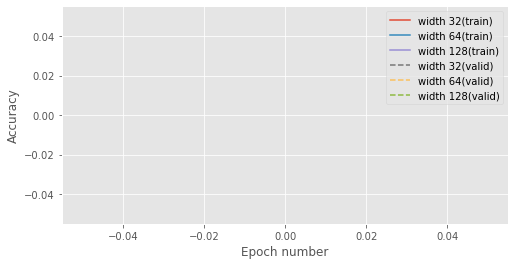
\includegraphics[width=\linewidth]{figures/empty_acc_curve_width.png}
        \caption{accuracy by epoch}
        \label{fig:width_acccurves}
    \end{subfigure} 
    \begin{subfigure}{\linewidth}
        \centering
        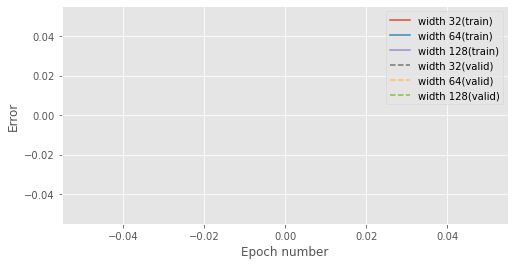
\includegraphics[width=\linewidth]{figures/empty_error_curve_width.png}
        \caption{error by epoch}
        \label{fig:width_errorcurves}
    \end{subfigure} 
    \caption{Training and validation curves in terms of classification accuracy (a) and cross-entropy error (b) on the EMNIST dataset for different network widths.}
    \label{fig:width}
\end{figure} 
}
}

%% Question Figure 3:
\newcommand{\questionFigureThree} {
\youranswer{Question Figure 3 - Replace these images with figures depicting the accuracy and error, training and validation curves for your experiments varying the number of hidden layers.
%
\begin{figure}[t]
    \centering
    \begin{subfigure}{\linewidth}
        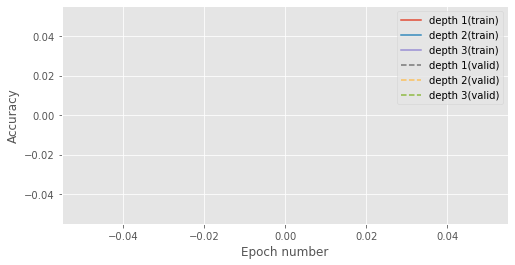
\includegraphics[width=\linewidth]{figures/empty_acc_curve_depth.png}
        \caption{accuracy by epoch}
        \label{fig:depth_acccurves}
    \end{subfigure} 
    \begin{subfigure}{\linewidth}
        \centering
        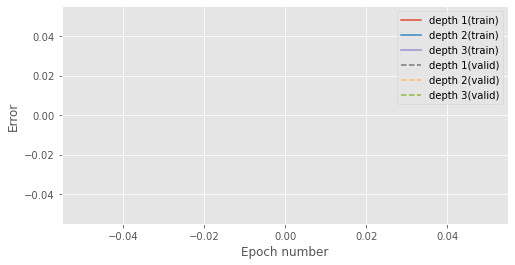
\includegraphics[width=\linewidth]{figures/empty_error_curve_depth.png}
        \caption{error by epoch}
        \label{fig:depth_errorcurves}
    \end{subfigure} 
    \caption{Training and validation curves in terms of classification accuracy (a) and cross-entropy error (b) on the EMNIST dataset for different network depths.}
    \label{fig:depth}
\end{figure} 
}
}

%% Question Figure 4:
\newcommand{\questionFigureFour} {
\youranswer{Question Figure 4 - Replace these images with figures depicting the Validation Accuracy and Generalisation Gap (difference between validation and training error) for each of the experiment results varying the Dropout inclusion rate, and L1/L2 weight penalty depicted in Table 3 (including any results you have filled in).
%
\begin{figure*}[t]
    \centering
    \begin{subfigure}{.475\linewidth}
        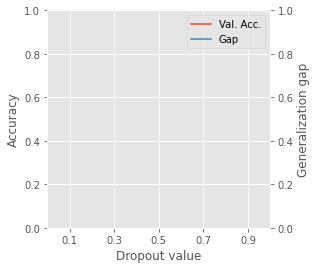
\includegraphics[width=\linewidth]{figures/empty_dropout_plot.png}
        \caption{Accuracy and error by inclusion probability.}
        \label{fig:dropoutrates}
    \end{subfigure} 
    \begin{subfigure}{.475\linewidth}
        \centering
        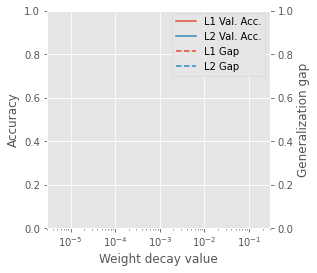
\includegraphics[width=\linewidth]{figures/empty_wd_plot.png}
        \caption{Accuracy and error by weight penalty.}
        \label{fig:weightrates}
    \end{subfigure} 
    \caption{Accuracy and error by regularisation strength of each method (Dropout and L1/L2 Regularisation).}
    \label{fig:hp_search}
\end{figure*}
}
}

%% - - - - - - - - - - - - TABLES - - - - - - - - - - - - 

%% Question Table 1:
\newcommand{\questionTableOne} {
\youranswer{
Question Table 1 - Fill in Table 1 with the results from your experiments varying the number of hidden units.
%
\begin{table}[t]
    \centering
    \begin{tabular}{c|ccc}
    \toprule
        \# Hidden Units & Val. Acc. & Train Error & Val. Error\\
    \midrule
         32            &    --.-   &  -.--- &   -.---            \\
         64            &    --.-   &  -.---  &   -.---               \\
         128           &    --.-   &  -.---  &   -.---           \\ 
    \bottomrule
    \end{tabular}
    \caption{Validation accuracy (\%) and training/validation error (in terms of cross-entropy error) for varying network widths on the EMNIST dataset.}
    \label{tab:width_exp}
\end{table}
}
}

%% Question Table 2:
\newcommand{\questionTableTwo} {
\youranswer{
Question Table 2 - Fill in Table 2 with the results from your experiments varying the number of hidden layers.
%
\begin{table}[t]
    \centering
    \begin{tabular}{c|ccc}
    \toprule
        \# Hidden Layers & Val. Acc. & Train Error & Val. Error \\
    \midrule
         1               &      --.-      &   -.--- & -.---                \\
         2               &      --.-      &   -.--- & -.---                \\
         3               &      --.-      &   -.--- & -.---                \\ 
    \bottomrule
    \end{tabular}
    \caption{Validation accuracy (\%) and training/validation error (in terms of cross-entropy error) for varying network depths on the EMNIST dataset.}
    \label{tab:depth_exps}
\end{table}
}
}

%% Question Table 3:
\newcommand{\questionTableThree} {
\youranswer{
Question Table 3 - Fill in Table 3 with the results from your experiments for the missing hyperparameter values for each of L1 regularisation, L2 regularisation, Dropout and label smoothing (use the values shown on the table).
%
\begin{table*}[t]
    \centering
    \begin{tabular}{c|c|ccc}
    \toprule
        Model    &  Hyperparameter value(s) & Validation accuracy & Train Error & Validation Error \\
    \midrule
    \midrule
        Baseline &  -                    &               0.837 &       0.241 &  0.533          \\
    \midrule
        \multirow{4}*{Dropout}
                 & 0.6                   &  80.7                &      0.549 & 0.593     \\
                 & 0.7 & --.- & -.--- & -.---  \\
                 & 0.85 & 85.1 &  0.329 &  0.434 \\
                 & 0.97 & 85.4 &  0.244 & 0.457  \\
    \midrule
        \multirow{4}*{L1 penalty}
                 & 5e-4 & 79.5 & 0.642 & 0.658 \\
                 & 1e-3 & --.- & -.--- & -.--- \\
                 & 5e-3 & 2.41 & 3.850 & 3.850 \\
                 & 5e-2 & 2.20 & 3.850 & 3.850 \\
    \midrule
        \multirow{4}*{L2 penalty}  
                 & 5e-4 & 85.1 & 0.306 & 0.460 \\
                 & 1e-3 & --.- & -.--- & -.--- \\
                 & 5e-3 & 81.3 & 0.586 & 0.607 \\
                 & 5e-2 & 39.2 & 2.258 & 2.256  \\
    \midrule
        Label smoothing & 0.1 & --.- & -.--- & -.--- \\
    \bottomrule
    \end{tabular}
    \caption{Results of all hyperparameter search experiments. \emph{italics} indicate the best results per series (Dropout, L1 Regularisation, L2 Regularisation, Label smoothing) and \textbf{bold} indicates the best overall.}
    \label{tab:hp_search}
\end{table*}
}
}

%% END of YOUR ANSWERS